% !TeX document-id = {4f147eee-d14c-456d-a180-f16d91e7a27a}
\documentclass[12pt, twoside, a4paper]{article}
% Following are the packages used for typsetting documents.
% More info on these packages at Comprehensive TeX Archive Network (CTAN) https://www.ctan.org/
\usepackage[top=1.333in, 
			bottom=0.666in,
			outer=0.633in,
			inner=1.466in,
			headsep=24pt]{geometry} % for setting the paper margins
			%
			%	 -------------------
			%	|		top			|	(top includes headsep)
			%	--------------------
			%	|	|			  | |
			%	| i	|			  |o|
			%	| n	|	 text	  |u|
			%	| n	|	 body	  |t|
			%	| e	|			  |e|
			%	| r	|			  |r|
			%	|	|			  | |
			%	---------------------
			%	|		bottom		|
			%	---------------------
			%
			% The dimensions for A4 paper are 8.5in x 11.0in.
			% Inner : outer = 1 : 2 textwidth set to 6.4 in (chosen such that 6 inch figure can fit in it without overfull.)
			% bottom : top = 1 : 2 textheight set to 9.0 in
			% The above dimensions for the margins leads to textbody dimensions of 6.4 in x 9.0 in.
\usepackage{graphicx}				% for handling floats/figures
\usepackage{caption}				% for special captioning in figure environment
\usepackage{subcaption}				% for subcaptioning in subfigure environment
\usepackage[usenames, dvipsnames]{xcolor}					% for handling colour
\usepackage{minted}					% for highlightling and formatting source code 
									% ALERT!!! minted needs shell-escape option for compile. Set
									% locally using following command 
									% Reference: https://tex.stackexchange.com/questions/99475/how-to-invoke-latex-with-the-shell-escape-flag-in-texstudio-former-texmakerx
% !TeX TXS-program:compile = txs:///pdflatex/[--shell-escape]
\usepackage[listings]{tcolorbox}	% for coloured and framed text boxes
\usepackage{amsmath}				% American Mathematical Society (AMS) defined mathmode
\usepackage{amssymb}				% AMS defined math symbols
\usepackage{siunitx}				% for si units
\usepackage[hidelinks,
			letterpaper,
			pagebackref,
			bookmarksopen,
			bookmarksnumbered,
			colorlinks = true,
			linkcolor = blue,
			urlcolor  = blue,
			citecolor = RoyalBlue,
			anchorcolor = blue]{hyperref}	% for hyperlinking
			% hyperref should always be at the last of the packages to be loaded!
\title{Documentation of Image Processing of Kerr micrographs}
\author{Sreekar, Ravi}
\date{\today}
\begin{document}
%
\maketitle
\cleardoublepage
\tableofcontents
\cleardoublepage
\section{Python virtual environment}
It is recommended that every new python project needs to be run in a separate \href{https://docs.python.org/3/tutorial/venv.html#creating-virtual-environments}{virtual environment}. There are various ways to maintain virtual environments. 
\begin{itemize}
	\item \href{https://docs.python.org/3/tutorial/venv.html#creating-virtual-environments}{venv} is a Python package to create virtual enviroment. Its low level and needs command line usage to configure the environment.
	\item \href{https://docs.anaconda.com/anaconda/install/windows/}{Anaconda} provides around 1500 packages in its default environment called base(root) and is useful for new Python users who do not want to meddle with installation issues. Its high level where Anaconda provides Graphical User Interface~(GUI) to manage the environments. However we can also  \href{https://docs.anaconda.com/anaconda/navigator/tutorials/create-python35-environment/?highlight=environment%20create#creating-a-python-3-5-environment-from-anaconda2-or-anaconda3}{set up a custom environment using Anaconda's Navigator}  
	\item \href{https://www.enthought.com/}{Enthought} way Another competitor to Anaconda.
	\item \href{https://docs.conda.io/en/latest/miniconda.html}{Miniconda} way is a smaller footprint version of Anaconda, which provides a minimal working base(root) Python environment. 
\end{itemize}
%
\subsection{Install Anaconda}
We will use Anaconda for our Kerr microscopy processing project. Once Anaconda is installed, a default environment called \textbf{base(root)} is created~(open Navigator). We need to create a new environmentc called \textbf{envKerr}. This is shown in \href{https://www.youtube.com/watch?v=8bzp04TeE3I}{YouTube video}. 

Now let us build the project in \textbf{envKerr}. A project is usually built on existing python packages. To install these packages, Anaconda provides a default channel from which we can download the packages. Scientific projects usually depend on the following core packages.
\begin{itemize}
	\item \href{https://docs.scipy.org/doc/numpy-1.13.0/reference/arrays.indexing.html#}{numpy} for handling arrays
	\item \href{https://docs.scipy.org/doc/scipy/reference/optimize.html}{scipy} for handling statistical computation
	\item \href{https://matplotlib.org/}{matplotlib} A good reference for  \href{https://github.com/rougier/matplotlib-tutorial}{matplotlib for researchers} can be a starting point.
\end{itemize}

Also in addition to the above packages, for image processing, we need the following packages.
\begin{itemize}
	\item \href{https://docs.opencv.org/trunk/d6/d00/tutorial_py_root.html}{openCV} open source package for Computer Vision~(CV). openCV handles almost all the image processing task and is used in various high end projects. It is originally implemented in the C programming language and is ``wrapped'' as a python package. Though it is a powerful package, it has a steep learning curve. Also due to C implementation, it is faster performance than python based implementations.
	\item \href{https://scikit-image.org/docs/dev/index.html}{scikit-image} is a pure python implementation for image processing. It has a shallow learning curve but limited in usage. For example, in our project, scikit-image has no routine for ellipse fitting. Also it is slower than openCV
\end{itemize}
We will use openCV for the image processing. \textcolor{red}{However Anaconda does not come preinstalled with opencv package in default installation.}  The procedure to install opencv in the custom \textbf{envKerr} enviroment is described the Youtube video. The default channel of Anaconda contains older stable versions of openCV. However if latest version is needed, they can be installed from \href{https://github.com/conda-forge}{\textbf{conda-forge}}. conda-forge is a channel maintained by a community consisting of researchers. Check the link on how to  \href{https://docs.anaconda.com/anaconda/navigator/tutorials/manage-channels/#adding-a-channel}{add conda-forge to Anaconda}. 

Finally we need an Integrated Development Environment~(IDE) for handling the Python files. An IDE provides the commonly need features for programming like
\begin{itemize}
	\item editor
	\item variable explorer
	\item console
	\item file explorer 
\end{itemize}
We will use spyder IDE for the project. spyder package is present in the default channel.
%
\subsection{Uninstall Anaconda}
Just with every other software, we need to know how to uninstall Anaconda. Though with most Windows based softwares, it is as easy as going to ``Add or Remove Programs'' and clicking Uninstall. However since Anaconda is developed for primarily for the GNU/Linux system, the \href{https://docs.anaconda.com/anaconda/install/uninstall/#}{uninstalling Anaconda} is a tricky procedure in Windows. \textcolor{red}{It is recommended to follow the above procedure} to avoid \href{https://www.howtogeek.com/314734/how-to-manually-remove-programs-from-the-windows-uninstall-program-list/}{phantom apps in the Windows Registry} as it is \textcolor{red}{\textbf{very risky}} to manually tweak the Registry files in order to remove these phantom apps.

\section{KerrPy}
The aim of a general image processing study is to extract ``image signal'' from ``image noise''. In our study, the image signal is a bubble domain having the geometrical characteristics of an ellipse, The image noise arises due to the way we capture/save the images.  The original raw image captured from the peltier cooled camera is a grayscale optical micrograph of the film surface. However when saving to the hard disk, we substract the image from a reference/background image. This is called background correction. Due to the background correction, there are two types of noise
%
\begin{itemize}
	\item salt and pepper noise
	\item drift noise due to topographical film defects
	\item ``amagnetic'' defects
\end{itemize}
%
Salt and pepper noise arises due to thermal noise. In an ideal scenario, this background correction should lead to an image with pixels of zero intensity. However, in a realistic scenario, there is an inherent noise of random nature associated with any measurement. Due to the noise, there is a fluctuation of pixel intensity about a baseline intensity. This is called \textbf{salt and pepper noise}. 

If there are topographical features like dust particles, they can get be removed from the image by background correction. However if there is a drift in the positioning of the sample, it can lead to reappearance of such features in the form of edges. This is called \textbf{drift noise}. It is to be noted that this can happen even if the topographical feature is part of the sample i.e. magnetic, for e.g, a patterned magnetic sample.

The other source of noise is due to ``amagnetic'' features like a defect in the film. If the bubble domain nucleates about the defect, even after substraction the defect can remain as unreversed in the substracted image.

Our project KerrPy consists of image processing routines for extraction of geometrical parameters of bubble domains from these sources of noise. These routines are based on openCV's transformation functions on images. The transformations critically depend on certain parameters which need to be optimized. The optimization varies on a problem to problem basis. As a result, these parameters need to be trained.
\subsection{Training the parameters}
Starting from the raw image, various transformations are applied as described below
\paragraph{Histogram equalization}
We take the raw image and apply histogram equalization. It leads to normalizing the intensity to full scale. This leads to separation of the peaks in the histogram as shown in Figure.~\ref{openCV histogram equalization}.
%
\begin{minted}[
frame=lines,
framesep=2mm,
baselinestretch=1.2,
bgcolor=lightgray,
fontsize=\footnotesize,
linenos
]{python}
equ = cv2.equalizeHist(img)

\end{minted}
%
%
\begin{figure}[!htbp]
	\centering
	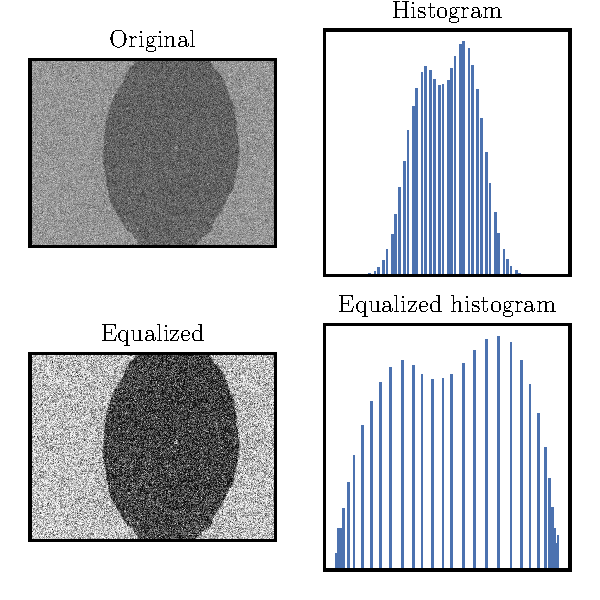
\includegraphics[scale=1.0]{figures/01_HistogramEqualizationEffect.pdf}
	\caption{Histogram equalization improves contrast allowing easier binarization of the image.
	}
	\label{openCV histogram equalization}
\end{figure}
%
\paragraph{Gaussian blurring}
We take the histogram equalized and apply Gaussian blur transformation. The Gaussian kernel size chosen is 5x5 pixels. Gaussian bluring leads to smoothening the salt and pepper noise and enhancement of the valley between the peaks of the histogram as shown in Figure.~\ref{openCV gaussian blurring}.
%
\begin{minted}[
frame=lines,
framesep=2mm,
baselinestretch=1.2,
bgcolor=lightgray,
fontsize=\footnotesize,
linenos
]{python}
blur = cv2.GaussianBlur(img,(5,5),0)
\end{minted}
%
%
\begin{figure}[!htbp]
	\centering
	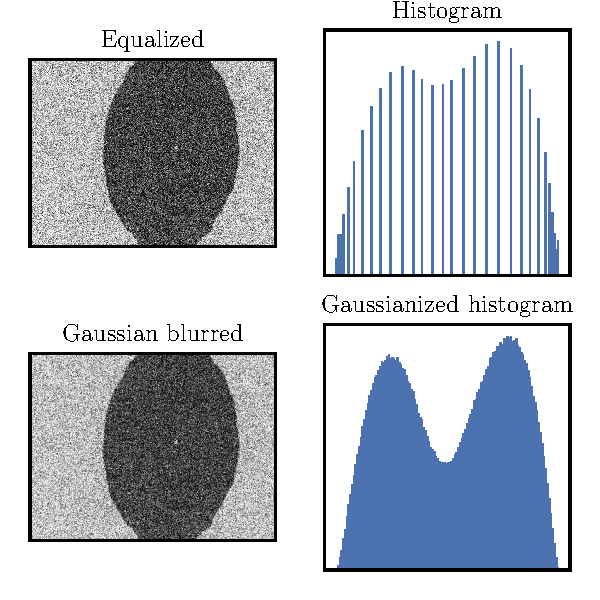
\includegraphics[scale=1.0]{figures/02_GaussianBlurringEffect.pdf}
	\caption{Guassian blurring enhances peak intensities of the binary images allowing easier binarization of the image.
	}
	\label{openCV gaussian blurring}
\end{figure}
%
\paragraph{Median filtering}
We take the Gaussian blurred image and apply median filtering transformation. The kernel for the transformation is again a 5x5 pixel window. Median filtering is most effective in reducing the salt and pepper noise as it reduces the width of the peaks. This is shown in Figure.~\ref{openCV median filtering}.
%
\begin{minted}[
frame=lines,
framesep=2mm,
baselinestretch=1.2,
bgcolor=lightgray,
fontsize=\footnotesize,
linenos
]{python}
median_blur= cv2.medianBlur(img,5)
\end{minted}
%
%
\begin{figure}[!htbp]
	\centering
	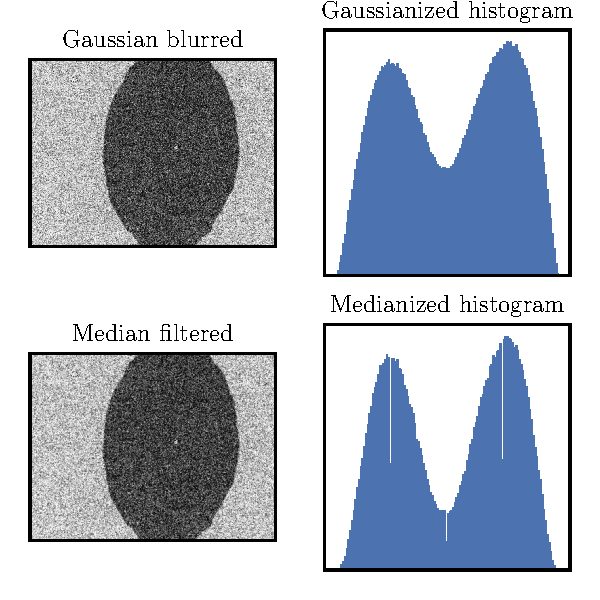
\includegraphics[scale=1.0]{figures/03_MedianFilteredEffect.pdf}
	\caption{Median filtering reduces the peak widths which is useful for reducing the salt and pepper noise.
	}
	\label{openCV median filtering}
\end{figure}
%
\paragraph{Otsu binarization}
Now that image is sufficiently processed for the reduction of salt and pepper noise, we apply binarization of the image with Otsu algorithm. Instead of the global threshold algorithm, Otsu binarization involves adaptive thresholding leading to overall better binarization. The results are shown in Figure.~\ref{openCV Otsu binarization}.
%
\begin{minted}[
frame=lines,
framesep=2mm,
baselinestretch=1.2,
bgcolor=lightgray,
fontsize=\footnotesize,
linenos
]{python}
ret, otsu = cv2.threshold(img,0,255,cv2.THRESH_BINARY+cv2.THRESH_OTSU)
\end{minted}
%
%
\begin{figure}[!htbp]
	\centering
	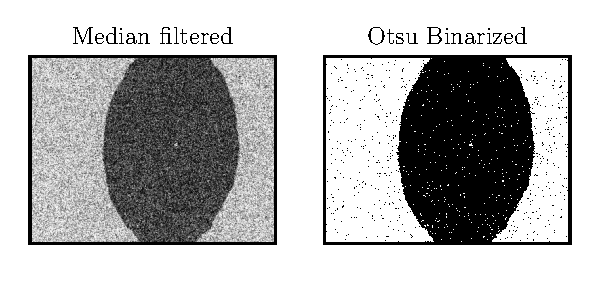
\includegraphics[scale=1.0]{figures/04_BinaryOtsuEffect.pdf}
	\caption{Otsu binarization involves finding an adaptive threshold.
	}
	\label{openCV Otsu binarization}
\end{figure}
%
\paragraph{Morphological transformation}
Binarization leads to formation of high contrast image. However it has speckles related to salt and pepper noise. If we define the white pixels as foreground and the dark pixels as background, then the small ``background islands'' in the foreground and ``foreground islands'' in the background are the so called speckles.  We need to remove the speckles using \href{https://docs.opencv.org/trunk/d9/d61/tutorial_py_morphological_ops.html}{morphological transformations} called erosion and dilation. 

Erosion is a transformation that shrinks the foreground(white). This leads to disappearance of speckles of the background~(black). However it also leads to shrinkage of the original domain~(foreground). To conserve the size of the domain, we need to apply dilation. Dilation is a transformation that expands the foreground~(white). The successive application of erosion and dilation is called \textbf{opening} where we retain the size of the foreground and removes the speckles(white type) in the background(black). 

Also the foreground~(white) contains speckles~(black type). To remove these speckes, we apply a similar successive application of dilation followed by erosion. This is called \textbf{closing}. Closing also retains the size of the object. The whole process of opening and closing is called morphological transformation as shown in Figure.~\ref{openCV erosion dilation}. 

Now the amount of shrinkage in erosion and expansion in dilation is set by the size of the kernel. We have used a kernel size of 9x9 pixels. Sometimes a second iteration of erosion and dilations is needed with a bigger kernel size to remove bigger speckles. However it is to be noted that bigger kernel size introduces distortions in the the object that can contribute to \textbf{processing induced noise}. A second iteration of 15x15 is performed to remove the bigger speckles. A direct step of bigger kernel size in the first iteration may worsen the situation. So it is observed an iterative procedure helps reduce the speckles.
%
\begin{minted}[
frame=lines,
framesep=2mm,
baselinestretch=1.2,
bgcolor=lightgray,
fontsize=\footnotesize,
linenos
]{python}
# morphological transformation i.e. opening and closing
# of the binary image to remove speckles

kernel = np.ones((9,9),np.uint8)

# erode the image and save
opened = cv2.morphologyEx(img, cv2.MORPH_OPEN, kernel)

# morphological transformation (two iterations; second iteration with bigger kernel 15) and save
openedthenclosed = cv2.morphologyEx(opened, cv2.MORPH_CLOSE, kernel)
\end{minted}
%
%
\begin{figure}[!htbp]
	\centering
	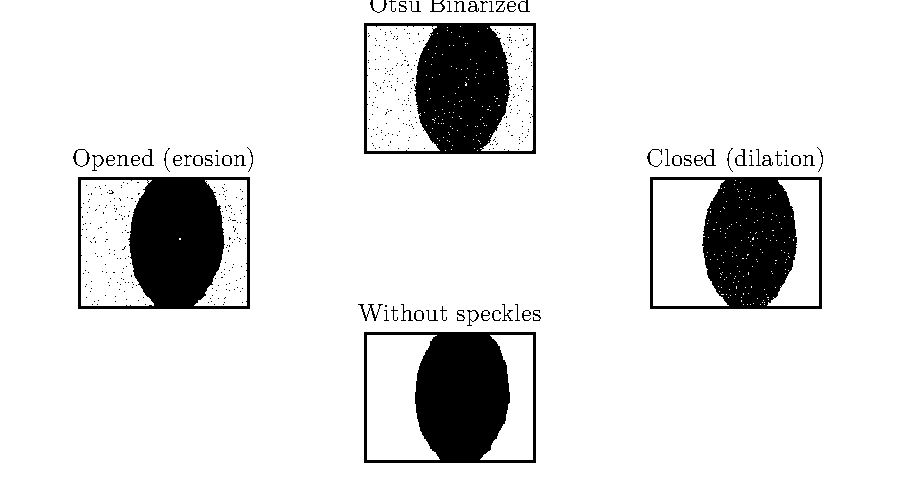
\includegraphics[scale=1.0]{figures/05_ErosionAndDilationEffect.pdf}
	\caption{Removal of speckles using erosion and dilation transformation.
	}
	\label{openCV erosion dilation}
\end{figure}
%
\paragraph{Canny edge detection}
Now we apply canny edge detection for detecting the edges of the ellipse. Canny edge algorithm works on the principle of joining the edges detecting using gradient transformation by providing two thresholds lower and upper. This is shown in Figure.~\ref{openCV canny edge}.
%
\begin{minted}[
frame=lines,
framesep=2mm,
baselinestretch=1.2,
bgcolor=lightgray,
fontsize=\footnotesize,
linenos
]{python}
#find the Canny edges
edges = cv2.Canny(img,100,200)
\end{minted}
%
%
\begin{figure}[!htbp]
	\centering
	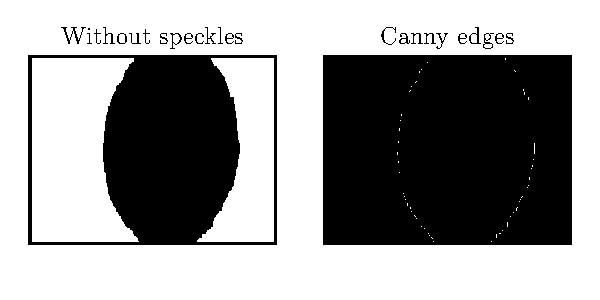
\includegraphics[scale=1.0]{figures/06_CannyEdgeEffect.pdf}
	\caption{Canny edge detection of domain wall profile.
	}
	\label{openCV canny edge}
\end{figure}
%
\paragraph{Adaptive ROI}
Due to the varying sizes of the domains as well as low contrast, we need to employ an adaptive ROI strategy to maximize the contrast between the domain and the background. We start with a ROI roughly centered around the nucleated bubble domain and increase the window size in subsequent steps. For each window size, a univariate modal analysis is performed on the histogram of the image as shown in Figure~\ref{openCV adaptive ROI big domain}. The optimum ROI is the one which can maximally resolve the peaks corresponding to the domain and background. For each ROI, the relative strength of the peaks, defined as the ratio of their intensities, is plotted. The optimum ROI is given by the maximum of the the relative strengths.
%
Using \textbf{Kernel Density Estimate}~(KDE) analysis, relative amount of foreground and background regions within a given ROI can be estimated. If the ROI is varied across the viewing area, an optimum relative strength can be found when the foreground and background area are nearly equal. This sets the value of adaptive threshold.
%
Since we know certain properties about our object of interest like the approximate center of object and the aspect ratio of object area, the ROI can be set accordingly
%
\begin{figure}[!htbp]
	\centering
	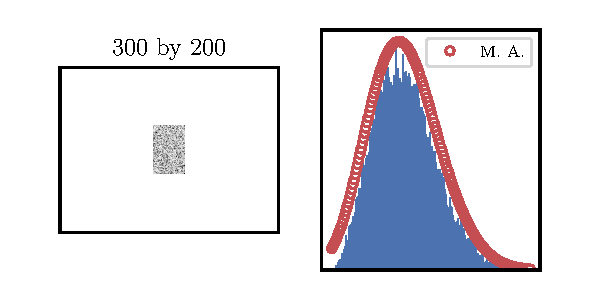
\includegraphics[scale=1.0]{figures/07_ModalAnalysisBigDomain/ModalAnalysis_xROI = 300 yROI = 200.pdf} \\
	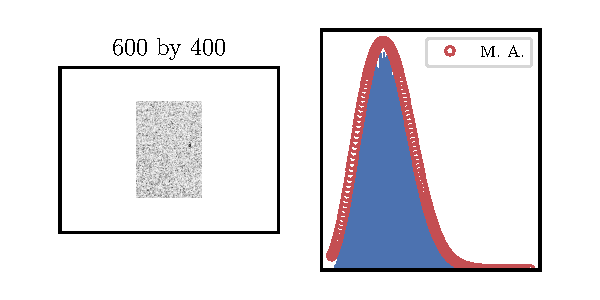
\includegraphics[scale=1.0]{figures/07_ModalAnalysisBigDomain/ModalAnalysis_xROI = 600 yROI = 400.pdf} \\
	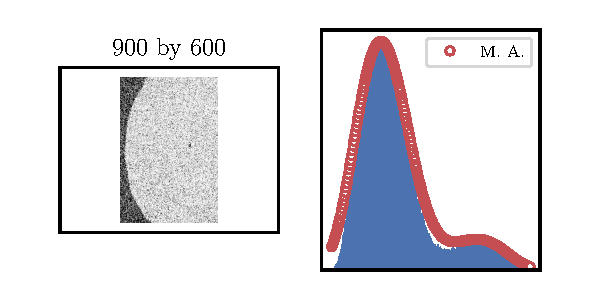
\includegraphics[scale=1.0]{figures/07_ModalAnalysisBigDomain/ModalAnalysis_xROI = 900 yROI = 600.pdf} \\
	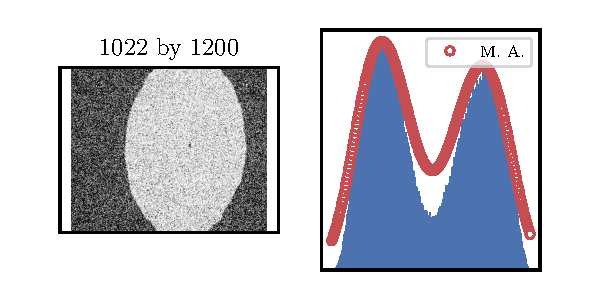
\includegraphics[scale=1.0]{figures/07_ModalAnalysisBigDomain/ModalAnalysis_xROI = 1022 yROI = 1200.pdf} \\
	\caption{Finding the optimum ROI by using an adaptive ROI algorithm and univariate modal analysis. For a big domain, the optimum ROI is the complete area 1022 by 1200 pixels.
	}
	\label{openCV adaptive ROI big domain}
\end{figure}
%
The algorithm works well even for a small domain as shown in Figure.~\ref{openCV adaptive ROI small domain}.
%
\begin{minted}[
frame=lines,
framesep=2mm,
baselinestretch=1.2,
bgcolor=lightgray,
fontsize=\footnotesize,
linenos
]{python}
def FitEllipse_LeastSquares(pnts):
'''
Simple least-squares ellipse fit to boundary points
Parameters
----
pnts : n x 2 array of integers
Candidate pupil-iris boundary points from edge detection
roi : 2D scalar array
Grayscale image of pupil-iris region for display only
cfg : configuration structure
Configuration parameters
Returns
----
best_ellipse : tuple of tuples
Best fitted ellipse parameters ((x0, y0), (a,b), theta)
'''

# Tiny circle init
best_ellipse = ((0,0),(1e-6,1e-6),0)

# Break if too few points to fit ellipse (RARE)
if pnts.shape[0] < 5:
return best_ellipse

# Call OpenCV ellipse fitting
best_ellipse = cv2.fitEllipse(pnts)

return best_ellipse
\end{minted}
%
%
\begin{figure}[!htbp]
	\centering
	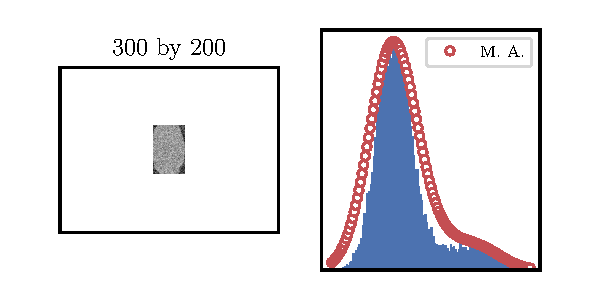
\includegraphics[scale=1.0]{figures/08_ModalAnalysisSmallDomain/ModalAnalysis_xROI = 300 yROI = 200.pdf} \\
	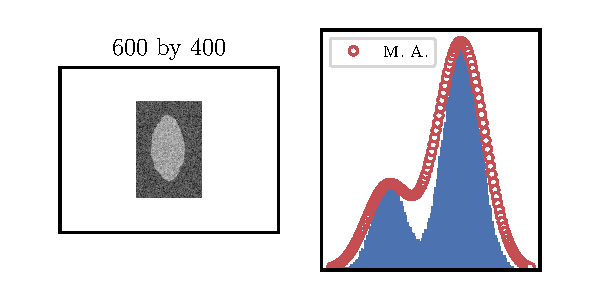
\includegraphics[scale=1.0]{figures/08_ModalAnalysisSmallDomain/ModalAnalysis_xROI = 600 yROI = 400.pdf} \\
	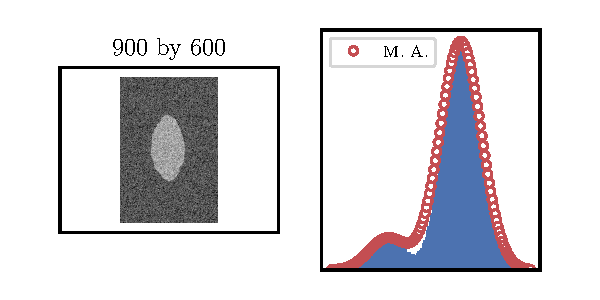
\includegraphics[scale=1.0]{figures/08_ModalAnalysisSmallDomain/ModalAnalysis_xROI = 900 yROI = 600.pdf} 
	\caption{Adaptive ROI algorithm works well for a small domain. The optimum ROI is 600 by 400 pixels.
	}
	\label{openCV adaptive ROI small domain}
\end{figure}
%
\paragraph{Training parameters}
So image processing needs training of the parameters. The parameters used for training are listed in Table with their sensitivity for image processing. Also the images have been captured at 20x magnfication with a wide area resolution of 1344 by 1066 pixels. For this magnfication, $\ldots$ corresponds to \SI{100}{\micro\metre}. Also the confidence of fit is defined heuristically by defining a maximum of the normalized error squared given by

Ellipse Fit Error function given by Swirski~\emph{et al.}~\cite{Swirski2012}
\begin{equation}
	content...
\end{equation}
\begin{table}
	\centering
	\begin{tabular}{lll}
		\hline\hline
		Parameter						& size 		& sensitivity 	\\
		\hline
		aspect ratio					& 2/3		& low			\\
		Gaussian kernel size			& 5 pixels 	& low			\\
		Median filtering kernel size	& 5 pixels	& high			\\
		erosion/dilation kernel size	& 9 pixels (first) 15 pixels (second)	& \textbf{very high}			\\
		Canny edge detection thresholds	& 100, 200	& high			\\
		\hline\hline
	\end{tabular}
	\caption{Training parameters for image processing.}
	\label{table training parameters}
\end{table}
%
\paragraph{Fitting ellipse}
We use ellipse fitting routine of OpenCV for fitting the ellipse. The routine uses Least Squares Fitting algorithm to obtain the fit. In addition to the fit, the the edge points lying away(or inside) a window of the fit are labelled as outliers(or inliers). According the fit, the inliers, and the outliers are respectively are represented by red green, blue respectively as shown in Figure.~\ref{openCV ellipse fits}. The concept of inliers and outliers is based on the work mrgaze by Mike Tyszka which are set of image processing routines for tracking pupil of the eye. MRGAZE provides scripts to perform offline pupilometry and gaze estimation from eyetracking video.~\cite{Tyszka2015}
%
\begin{figure}[!htbp]
	\centering
	\includegraphics[width=3in]{figures/09_FitEllipse/img1/RawImage.png}
	\includegraphics[width=3in]{figures/09_FitEllipse/img1/FitEllipse.png}\\
	\includegraphics[width=3in]{figures/09_FitEllipse/img2/RawImage.png}
	\includegraphics[width=3in]{figures/09_FitEllipse/img2/FitEllipse.png} \\
	\includegraphics[width=3in]{figures/09_FitEllipse/img3/RawImage.png}
	\includegraphics[width=3in]{figures/09_FitEllipse/img3/FitEllipse.png} \\		\includegraphics[width=3in]{figures/09_FitEllipse/img4/RawImage.png}
	\includegraphics[width=3in]{figures/09_FitEllipse/img4/FitEllipse.png}
	\caption{Bubble expansion and ellipse fits.
	}
	\label{openCV ellipse fits}
\end{figure}
%
%
\begin{figure}[!htbp]
	\centering
	\includegraphics[width=1.0\linewidth]{figures/09_FitEllipse/fitEllipsesSingle.png}
	\caption{Fit ellipses in single frame.
	}
	\label{openCV fit ellipses single frame}
\end{figure}
%
\paragraph{Fit parameters}
For a particular value of out of plane field $H_{z}$ and in plane field $H_{x}$, we pulse the $H_{z}$ for a sequence of $n_{\mathrm{Images}}$. For this sequence, we set a minimum confidence of $80\%$. For a fit less than the minimum confidence, we discard the fit. In Figure.~\ref{openCV fits parameters} , we plot the confidence, center X , center Y, semi major and semi minor axis and orientation for $H_z = -22~\mathrm{Oe}, H_x = 0~\mathrm{Oe}$. These are achieved from the program via running in the main program.
%
\clearpage
\subsection{Structure of raw data}
Vineeth's Labview program arranges the data in a way that separates the out of plane field from inplane fields. Irrespective of how the data is stored, let us bring some uniformity in the data. For this let us define the following terms
%
\begin{tcolorbox}[ title = Space, colback = red!5!white, colframe = red!75!black, colbacktitle=red!25!white]
	An space is defined as the ``area'' covered by the experiments that are performed over various values of $H_{z}, H_{x}, \Delta t$. 
	\tcblower
	NUCLEATE-M\_IPBHx0.00\_Ip-1.00E+1\_tp6.50E+3\_DUR CYC5 \\
	NUCLEATE-M\_IPBHx0.00\_Ip-1.20E+1\_tp2.50E+3\_DUR CYC5 \\
	NUCLEATE-M\_IPBHx0.00\_Ip-1.40E+1\_tp1.20E+3\_DUR CYC5
\end{tcolorbox}
%
%
\begin{tcolorbox}[ title = Experiment, colback = red!5!white, colframe = red!75!black, colbacktitle=red!25!white]
An experiment is defined primarily by the three parameters $H_{z}, H_{x}, \Delta t$. The other secondary parameters are nucleation(up or down). The data corresponding to an experiment is saved as folder with the foldername describing these parameters as shown below.
\tcblower
	ItNo1\_NUCLEATE-M\_IPBHx0.00\_Ip-1.00E+1\_tp6.50E+3\_DUR CYC5
\end{tcolorbox}
%
%
\begin{tcolorbox}[ title = Iteration, colback = red!5!white, colframe = red!75!black, colbacktitle=red!25!white]
	An iteration of an experiment is defined, in addition to the parameters of the experiment, by the index of iteration, for e.g. ItNo1. Each experiment can be run for few iterations to account for statistics. This is captured as iteration of an experiment. Each iteration contains a sequence of pulses set by the number of Pulses. Also it contains the inital saturation and final saturation for reference.
	\tcblower
	10\_-10.0000\_6500.000000.png \\
	11\_-10.0000\_6500.000000.png \\
	12\_-10.0000\_6500.000000.png \\
	INITIALUP SATURATION.png
\end{tcolorbox}
%
%
\begin{tcolorbox}[ title = Pulse, colback = red!5!white, colframe = red!75!black, colbacktitle=red!25!white]
	An pulse is defined by the actual execution of the parameters and is recorded with filename containing the iteration number starting from 10, out-plane field and pulse width.
	\tcblower
	10\_-10.0000\_6500.000000.png
\end{tcolorbox}
%

As can be seen from the structure of the data, it has heirarchial nature with the topmost level at the raw data and the bottom most at the pulse. To bring uniformity to the data, let us do some preconditioning
\subsubsection{Preconditioning}
From LabView program we get the sequence of experiments as shown in Figure.~. Let us save this experiment sequence to .csv file given by global variable \textbf{seq\_file}. Also club all the experiments in one folder RawData given by global variable \textbf{raw\_dir}. With this preconditioning of data, the data structure should like something like
\begin{verbatim}
Space
|
--- Experiment 0
       |
       --- Iteration 0
                     |
                     --- Pulse 0.png
                     --- Pulse 1.png
                     --- Initial ...
       --- Iteration 1 
       				 |
       				 --- Pulse 0.png
       				 --- Pulse 1.png
       				 --- Initial ...
--- Experiment 1
        |
        --- 
...

/\      /\       /\            /\
L0      L1       L2            L3
\end{verbatim}
%
\begin{itemize}
	\item \textcolor{red}{It is recommended to have the same number of pulses and same number of iterations across all the experiments.}. Otherwise the program might break.
	\item  To the traverse the above data structure heirarchy, we need two variables for each level; \textbf{level\_dir} for tracking the folder location and \textbf{level\_index} for the folder number.
	\item  Also the total number of folders in each level is also important to terminate the loop. This variable is given by \textbf{level\_iterations}.
\end{itemize}
The variables used for the various levels in the program are summarized in Table.~\ref{table: structure of data}.
%
\begin{table}[!htbp]
	\centering
	\begin{tabular}{lllll}
		\hline\hline
		Data folder			& Level & 	level\_variable	&	level\_index	&	level\_iterations	\\
		\hline
		space				&	0  	& 	raw\_dir	&	-- 		&	--	\\
		Experiment			&	1	&	exp\_dir	&	exp\_index	&	n\_exp	\\
		Iteration		 	&	2	&	iter\_dir	&	iter\_index	&	n\_iter	\\
		Pulse				&	3	&	img\_file	&	pulse\_index &	n\_pulse	\\
		\hline \hline
	\end{tabular}
	\caption{The levels of data structure and the corresponding variables used for program.}
	\label{table: structure of data}
\end{table}
\subsubsection{Handling spaces}
\paragraph{Full space}
Let us take a concrete example for understanding the data structure and fits structures.After we preconditioned the raw data as shown below, the directory should be placed in the parent directory.
%
\begin{minted}[
frame=lines,
framesep=2mm,
baselinestretch=1.2,
bgcolor=lightgray,
fontsize=\footnotesize,
linenos
]{python}
os.listdir()
Out[139]: 
['NUCLEATE-M_IPBHx0.00_Ip-1.00E+1_tp6.50E+3_DUR CYC5',
'NUCLEATE-M_IPBHx0.00_Ip-2.00E+1_tp3.00E+2_DUR CYC5']
\end{minted}
%
the experiment sequence TestSequence.csv used for generating the data is also placed in the parent directory and is given by
\begin{verbatim}
Current	PulseWidth	Pulse No	Dur Cyc	Ip Bias	Sampling	DAQ Time
-20	300	8	5	0	0	5
-10	6500	8	5	0	0	5
\end{verbatim}
%
Now from this .csv, total number of experiments = 2. We set the global variable \textbf{nImages}=9. Though it is not mentioned in this .csv, the number of iterations for each experiment is 1. Also each pulse gives an array of 6 parameters corresponding to confidence, major, minor, x-center and y-center. The shapes of the arrays for each of the params are given by Table.~\ref{table: shape of arrays of parameters}.

%
\begin{table}[!htbp]
	\centering
	\begin{tabular}{ll}
		\hline\hline
		parameter	&	 shape	 \\
		\hline
		$s$		&	$(2,1,1,6)$	\\
		$e$		& 	$(1,1,6)$ 	\\
		$i$		&	$(1, 6)$			\\
		$p$		&	$(6,)$				\\
		\hline\hline
	\end{tabular}
	\caption{Shapes of arrays of parameters.}
	\label{table: shape of arrays of parameters}
\end{table}


\paragraph{Custom space}
We can ``slice'' a part of the total space of experiments and perform custom processing. If the complete space is given by the experiments
Then to perform experiment on lets say last five experiments, we use following sequence file
\begin{verbatim}
Current	PulseWidth	Pulse No	Dur Cyc	Ip Bias	Sampling	DAQ Time
-20	300	8	5	0	0	5
\end{verbatim}
%
\subsection{Structure of program}
\begin{verbatim}
ParentDir
|
|--- KerrPy
|      |
|      --- Training
|      |
|      |
|      --- HandlingFile
|      |     |
|      |      --- processSpace.py
|      |      --- processExperiment.py
|      |      --- processIteration.py
|      |      --- processPulse.py
|      |
|      --- HandlingImage
|      |       |
|      |       |--- processOpenCV.py
|      |       |--- routinesOpenCV.py
|      |       |--- processROI.py
|      |       |--- fitEllipse.py
|      |
|      --- HandlingStatistics
|      |        |
|      |        --- routinesSciPy.py
|      |
|      --- HandlingFigure
|      |         |
|      |         --- routinesMatplotlib.py              
|      |
|      |--- globalVariables.py
|      |--- processFits.py
|      |--- loadFits.py
|      |--- plotFits.py      
|
|--- DataSimplified
|--- DataTraining
|--- PostProcessing
       |
       |--- Fits
       |--- Images
\end{verbatim}
%
The \textbf{KerrPy} program files are placed in parent directory~\textbf{ParentDir}. KerrPy is comprised mainly of three scripts
\begin{itemize}
	\item processFits.py
	\item loadFits.py
	\item plotFits.py
\end{itemize}
These scripts depend on mainly on four types of scripts
\begin{itemize}
	\item globalVariables.py 
	\item HandlingFile 
	\item HandlingImage
	\item HandlingStatistics
	\item HandlingFigure
\end{itemize}
globalVariables.py is for setting the parameters for processing. HandlingFile contains scripts for file handling operations based on operating system routines of standard Python package \textbf{os}. HandlingImage contains script for image processing operations based on routines of \textbf{openCV}. The images are handled as 2D \textbf{numpy} arrays. HandlingStatistics contains script for performing univariate modal analysis on image histogram based on routines of \textbf{scipy}. HandlingFigure contains script for plotting figures using \textbf{matplotlib}.
starts at main(). Main calls the subroutines in a heirarchial way to mimic the heiracharial arrangment of raw data. There are four levels of subroutines summarized in Table.~\ref{table: structure of program}. 
%
\begin{table}[!htbp]
	\centering
	\begin{tabular}{ll}
		\hline\hline
		subroutine	&	 extracts	 \\
		\hline
		processControls()		&	$[[H_{x0}, H_{z0}, \Delta t_{0}], [H_{x1}, H_{z1}, \Delta t_{1}], \ldots]$	\\
		processSpace(controls)	& 	$s = [e_{0}, e_{1}, \ldots]$ 	\\
		processExperiment(exp\_index, exp\_dir)		&	$e = [i_{0}, i_{1}, \ldots]$			\\
		processIteration(iter\_index, exp\_index, iter\_dir)	&	$i = [p_{0}, p_{1}, \ldots]$				\\
		processPulse(pulse\_index, iter\_index, exp\_index, img\_file)	&	$p = [c, a, b, x_{c}, y_{c}, o]$			\\
		\hline\hline
	\end{tabular}
	\caption{Extraction of parameters at each level using corresponding subroutines. Note that separate arrays are maintained for each of the paramters: confidence~$c$, semi-major axis~$a$, semi-minor axis~$b$, x-center~$x_{c}$, y-center~$c, a, b, x_{c}, y_{c}, o$ and orientation. So each level adds new dimension to the array used for storing these parameters.}
	\label{table: structure of program}
\end{table}
%
To understand the structure of the program and that of the extracts, we need to look at a concrete example which involves running two scripts
\begin{itemize}
	\item processFits.py
	\item loadFits.py
\end{itemize}

\subsubsection{Global parameters}
\paragraph{File handling parameters}
Now to save the parameters and images of fits, we need a processing directory given by global variable \textbf{proc\_dir}. Sometimes images may not be needed and we want to store only the parameters. So separate subdirectories for images and fits within the processing directory are present and given respectively by global variables \textbf{imgs\_folder} and \textbf{fits\_folder}. Each sample can have its own folder within the processing dir. For this we use global variable \textbf{samplename}. Finally the arrays corresponding to controls and the params are stored using the global variables \textbf{save\_controls\_file} and \textbf{save\_exps\_file}.
%
\begin{minted}[
frame=lines,
framesep=2mm,
baselinestretch=1.2,
bgcolor=lightgray,
fontsize=\footnotesize,
linenos
]{python}
##########################
##file handling parameters
##########################.
raw_dir = r'DataSimplified'
proc_dir = r'PostProcessing'
imgs_folder = r'Images'
fits_folder = r'Fits'
seq_file = r'testSequence.csv'
samplename = r'DataSimplified'

save_exps_file = 'space.npy'
save_controls_file = 'controls.npy'
\end{minted}

\paragraph{Debug parameters}
To enable or disable saving images, we have global flag \textbf{saveImages}. Also for training the parameters, we need to visualize images. To enable or disable display images, we have global flag \textbf{displayImages}. For debugging, we have \textbf{debug} and \textbf{deep\_debug} global flags.
%
\begin{minted}[
frame=lines,
framesep=2mm,
baselinestretch=1.2,
bgcolor=lightgray,
fontsize=\footnotesize,
linenos
]{python}
#########################
######debug parameters###
#########################
debug = True
deep_debug = False
displayImages = False
saveImages = True
\end{minted}
%
\paragraph{Training parameters}

\begin{minted}[
frame=lines,
framesep=2mm,
baselinestretch=1.2,
bgcolor=lightgray,
fontsize=\footnotesize,
linenos
]{python}
#######################
##training parameters##
#######################
nucleation_down =   True       # False for nucleation up
nImages         =   9       # number of pulses in an iteration
center_ROI      =   (511,672)  #center of the object to be identified
adaptive_ROI    =   True    # flag for adaptive ROI
aspr_ROI        =   2/3     # x_width/y_width for zooming out ROI.
# will be used if adaptive_ROI is True
kernel_gaussian =   5       # kernel for blurring !should be ODD
# typical values 3, 5, 7
kernel_median   =   5       # kernel for median filtering ! should be ODD
# typical values 3, 5, 7
kernel_speckless=   9       # kernel for opening and closing! should be ODD
# typical values 7, 9, 11
kernel_speckless_second = 15    # second level opening and closing
# ! should be ODD
max_norm_err_sq =   20.0    # maximum allowed normalized error
# allowed for a point to be an inlier
min_confidence  =   40.0    # minimum confidence for fit to be considered OK
\end{minted}
%


\subsubsection{processSpace()}
We get the experiments and controls from this subroutine. The controls corresponding to these experiments are 
\begin{minted}[
frame=lines,
framesep=2mm,
baselinestretch=1.2,
bgcolor=lightgray,
fontsize=\footnotesize,
linenos
]{python}
controls
Out[150]: 
array([['0.0', '-20.0', '300.0'],
['0.0', '-10.0', '6500.0']], dtype='<U6')
\end{minted}

whereas the experiments have shape
\begin{minted}[
frame=lines,
framesep=2mm,
baselinestretch=1.2,
bgcolor=lightgray,
fontsize=\footnotesize,
linenos
]{python}
space.shape
Out[148]: (2, 1, 9, 6)
\end{minted}

\subsubsection{processExperiment()}
The following is the code for processExperiment(). 
\begin{minted}[
frame=lines,
framesep=2mm,
baselinestretch=1.2,
bgcolor=lightgray,
fontsize=\footnotesize,
linenos
]{python}
def processExperiment(exp_index, exp_dir):
"""
LEVEL 1
0. Enter the experiment directory
1. Scan through the iterations
2. Return the experiments
"""

if debug: print("    L1 processExperiment() started at E:{exp_index}")

#Store the current location before relocating
cur_path = os.path.abspath(os.curdir)

# enter the experiment directory Level 1
os.chdir(exp_dir)


# initialize a list for saving iterations
experiment = []

files = os.listdir()
iter_dirs = [each for each in files if os.path.isdir(each)]
iter_dirs.sort()

for i, iter_dir in enumerate(iter_dirs):
iter_index = i
iteration = processIteration(iter_index, exp_index, iter_dir)
experiment.append(iteration)

#save the iterations to file    
saveExperiment(exp_index, experiment)

#Restore the path
os.chdir(cur_path)

return experiment
\end{minted}
%
Now to get the details about the  experiment 0 we use
\begin{minted}[
frame=lines,
framesep=2mm,
baselinestretch=1.2,
bgcolor=lightgray,
fontsize=\footnotesize,
linenos
]{python}
space[0]
Out[151]: 
array([[[   2.73354296,  516.90179443,  673.5869751 ,  992.12255859,
1348.75512695,    2.96985149],
[  99.61165049,  507.22918701,  667.29052734,  104.93482208,
181.13700867,   92.6811142 ],
[  91.56804734,  509.20106506,  666.59941101,  127.13392639,
237.81141663,   89.72157288],
[  72.09302326,  507.25747681,  666.15233612,  158.09284973,
293.30157471,   90.11330414],
[  79.08629442,  505.39341736,  666.56131744,  184.23310852,
354.30249023,   90.60331726],
[  72.36051502,  505.45350647,  666.5269928 ,  213.71313477,
410.78637695,   90.51153564],
[  69.84615385,  505.55145264,  666.08146667,  240.60980225,
468.07373047,   90.66560364],
[  62.22664016,  504.18157959,  664.05172729,  269.10467529,
529.98394775,   90.50309753],
[  61.6194865 ,  506.57528687,  663.79438782,  298.56863403,
578.6385498 ,   90.37406158]]])
\end{minted}
%
\subsubsection{processIteration()}
The code structure for processIteration() is similar to processExperiment(). Except there is one additional tracking variable \textbf{iter\_index} Since only one iteration is performed for each experiment, the size of the iteration dimension is 1.  We get the same information except that one level of nesting is reduced. The information of iteration 0 of the  experiment 0 can be accessed two ways as shown below.
\begin{minted}[
frame=lines,
framesep=2mm,
baselinestretch=1.2,
bgcolor=lightgray,
fontsize=\footnotesize,
linenos
]{python}
space[0][0]
Out[152]: 
array([[   2.73354296,  516.90179443,  673.5869751 ,  992.12255859,
1348.75512695,    2.96985149],
...
...
[  61.6194865 ,  506.57528687,  663.79438782,  298.56863403,
578.6385498 ,   90.37406158]])


space[0,0,:,:]
Out[153]: 
array([[   2.73354296,  516.90179443,  673.5869751 ,  992.12255859,
1348.75512695,    2.96985149],
...
...
[  61.6194865 ,  506.57528687,  663.79438782,  298.56863403,
578.6385498 ,   90.37406158]])
\end{minted}


\subsubsection{processPulse()}
Again the code structure for processPulse() is similar to processIteration() except there is one additional tracking variable \textbf{pulse\_index}. For example to get the  fits $c, a, b, x_c, y_c, o$ for Image 4 of Iteration 0 of Experiment 0 we use
\begin{minted}[
frame=lines,
framesep=2mm,
baselinestretch=1.2,
bgcolor=lightgray,
fontsize=\footnotesize,
linenos
]{python}
space[0][0][4]
Out[156]: 
array([ 79.08629442, 505.39341736, 666.56131744, 184.23310852,
354.30249023,  90.60331726])
\end{minted}
However if we want the confidence for all the images Iteration 0 of Experiment 1, we use
\begin{minted}[
frame=lines,
framesep=2mm,
baselinestretch=1.2,
bgcolor=lightgray,
fontsize=\footnotesize,
linenos
]{python}
space[1,0,:,0]
Out[159]: 
array([ 2.84605433, 99.82905983, 91.65526676, 95.05494505, 80.83416087,
71.98723065, 63.97058824, 72.21852099, 76.66480134])
\end{minted}
\subsection{Scripts}
\subsubsection{trainingParameters.py}
trainingParameters.py trains the image processing parameters. User intervention is needed to fine tune the parameters.
\subsubsection{processFits.py}
The output of processFits.py is given by
\begin{minted}{python}
runfile('E:/MonthlyWork/Y20/M09/RaviKumarWork/KerrPy-master/processFits.py', wdir='E:/MonthlyWork/Y20/M09/RaviKumarWork/KerrPy-master')
L0 processControls() started
number of experiments is 2
Control Knobs for experiments are 
[['0.0', '-66.0', '50.0'], ['50.0', '-66.0', '40.5']]
L0 saveControls() started
L0 processSpace() started
L0 E: 0 = ['0.0', '-66.0', '50.0']
extracted controls: ['0.0', '-66.0', '50.0']
L1 processExperiment() started at E: 0
L2 processIteration() started at E:0 I:0
L3 processPulse() started at E:0 I:0 P:0
U. A. peaks: [124.] at [100, 100]
U. A. peaks: [126.] at [200, 200]
U. A. peaks: [  8. 127. 242.] at [300, 300]
U. A. peaks: [  6. 127. 247.] at [400, 400]
U. A. peaks: [  6. 127. 249.] at [500, 500]
U. A. peaks: [  6. 127. 251.] at [600, 600]
U. A. peaks: [  5. 127. 251.] at [700, 700]
U. A. peaks: [  5. 127. 252.] at [800, 800]
max_rel_strength: 0.00
Opt ROI: (800, 800)
n_edges: 28
c(fit): 6%
img_color.shape: (800, 800, 3)
L3 saveImage() started at E:0 I:0 P:0
L3 savePulse() started at E:0 I:0 P:0
L3 processPulse() started at E:0 I:0 P:1
U. A. peaks: [112.] at [100, 100]
U. A. peaks: [143.] at [200, 200]
U. A. peaks: [136. 241.] at [300, 300]
U. A. peaks: [  8. 132. 246.] at [400, 400]
U. A. peaks: [  7. 130. 249.] at [500, 500]
U. A. peaks: [  6. 129. 251.] at [600, 600]
U. A. peaks: [  5. 129. 252.] at [700, 700]
U. A. peaks: [  5. 129. 252.] at [800, 800]
max_rel_strength: 0.00
Opt ROI: (300, 300)
n_edges: 2
c(fit): 95%
img_color.shape: (300, 300, 3)
L3 saveImage() started at E:0 I:0 P:1
L3 savePulse() started at E:0 I:0 P:1
L3 processPulse() started at E:0 I:0 P:2
U. A. peaks: [113.] at [100, 100]
U. A. peaks: [ 11. 115.] at [200, 200]
U. A. peaks: [ 99. 153.] at [300, 300]
U. A. peaks: [ 86. 143.] at [400, 400]
U. A. peaks: [ 79. 138. 243.] at [500, 500]
U. A. peaks: [ 75. 134. 250.] at [600, 600]
U. A. peaks: [  7.  72. 133. 251.] at [700, 700]
U. A. peaks: [  6.  70. 131. 251.] at [800, 800]
max_rel_strength: 0.79
Opt ROI: (300, 300)
n_edges: 3
c(fit): 86%
img_color.shape: (300, 300, 3)
L3 saveImage() started at E:0 I:0 P:2
L3 savePulse() started at E:0 I:0 P:2
L3 processPulse() started at E:0 I:0 P:3
U. A. peaks: [113.] at [100, 100]
U. A. peaks: [  9. 118.] at [200, 200]
U. A. peaks: [  7. 116.] at [300, 300]
U. A. peaks: [101. 162.] at [400, 400]
U. A. peaks: [ 88. 150.] at [500, 500]
U. A. peaks: [ 81. 143. 248.] at [600, 600]
U. A. peaks: [ 76. 139. 250.] at [700, 700]
U. A. peaks: [ 73. 136. 251.] at [800, 800]
max_rel_strength: 0.77
Opt ROI: (500, 500)
n_edges: 4
c(fit): 85%
img_color.shape: (500, 500, 3)
L3 saveImage() started at E:0 I:0 P:3
L3 savePulse() started at E:0 I:0 P:3
L3 processPulse() started at E:0 I:0 P:4
U. A. peaks: [114.] at [100, 100]
U. A. peaks: [  8. 117.] at [200, 200]
U. A. peaks: [  5. 118.] at [300, 300]
U. A. peaks: [  5. 115.] at [400, 400]
U. A. peaks: [ 12. 104. 165.] at [500, 500]
U. A. peaks: [ 92. 155. 247.] at [600, 600]
U. A. peaks: [ 84. 148. 248.] at [700, 700]
U. A. peaks: [ 79. 143. 249.] at [800, 800]
max_rel_strength: 0.01
Opt ROI: (200, 200)
n_edges: 5
c(fit): 32%
img_color.shape: (200, 200, 3)
L3 saveImage() started at E:0 I:0 P:4
L3 savePulse() started at E:0 I:0 P:4
L3 processPulse() started at E:0 I:0 P:5
U. A. peaks: [112.] at [100, 100]
U. A. peaks: [  8. 117.] at [200, 200]
U. A. peaks: [  5. 118. 243.] at [300, 300]
U. A. peaks: [  4. 119. 247.] at [400, 400]
U. A. peaks: [  6. 115. 245.] at [500, 500]
U. A. peaks: [ 10. 105. 167. 249.] at [600, 600]
U. A. peaks: [ 94. 158. 248.] at [700, 700]
U. A. peaks: [ 87. 151. 249.] at [800, 800]
max_rel_strength: 0.01
Opt ROI: (200, 200)
n_edges: 4
c(fit): 76%
img_color.shape: (200, 200, 3)
L3 saveImage() started at E:0 I:0 P:5
L3 savePulse() started at E:0 I:0 P:5
L2 saveIteration() started at E:0 I:0
L1 saveExperiment() started at E: 0
L0 E: 1 = ['50.0', '-66.0', '40.5']
extracted controls: ['0.0', '-66.0', '50.0']
extracted controls: ['50.0', '-66.0', '40.5']
L1 processExperiment() started at E: 1
L2 processIteration() started at E:1 I:0
L3 processPulse() started at E:1 I:0 P:0
U. A. peaks: [125.] at [100, 100]
U. A. peaks: [126.] at [200, 200]
U. A. peaks: [  6. 127. 247.] at [300, 300]
U. A. peaks: [  5. 127. 250.] at [400, 400]
U. A. peaks: [  4. 127. 248.] at [500, 500]
U. A. peaks: [  4. 126. 251.] at [600, 600]
U. A. peaks: [  4. 127. 251.] at [700, 700]
U. A. peaks: [  4. 127. 205. 251.] at [800, 800]
max_rel_strength: 0.00
Opt ROI: (800, 800)
n_edges: 16
c(fit): 10%
img_color.shape: (800, 800, 3)
L3 saveImage() started at E:1 I:0 P:0
L3 savePulse() started at E:1 I:0 P:0
L3 processPulse() started at E:1 I:0 P:1
U. A. peaks: [105.58823529] at [100, 100]
U. A. peaks: [136.] at [200, 200]
U. A. peaks: [131.] at [300, 300]
U. A. peaks: [  9. 130. 248.] at [400, 400]
U. A. peaks: [  7. 128. 249.] at [500, 500]
U. A. peaks: [  6. 128. 251.] at [600, 600]
U. A. peaks: [  5. 128. 251.] at [700, 700]
U. A. peaks: [  4. 127. 252.] at [800, 800]
max_rel_strength: 0.00
Opt ROI: (800, 800)
n_edges: 41
c(fit): 8%
img_color.shape: (800, 800, 3)
L3 saveImage() started at E:1 I:0 P:1
L3 savePulse() started at E:1 I:0 P:1
L3 processPulse() started at E:1 I:0 P:2
U. A. peaks: [112.] at [100, 100]
U. A. peaks: [104.] at [200, 200]
U. A. peaks: [ 90. 143.] at [300, 300]
U. A. peaks: [ 80. 136. 245.] at [400, 400]
U. A. peaks: [ 74. 133. 247.] at [500, 500]
U. A. peaks: [  7.  71. 131. 250.] at [600, 600]
U. A. peaks: [  5.  69. 130. 251.] at [700, 700]
U. A. peaks: [  5.  68. 129. 251.] at [800, 800]
max_rel_strength: 0.52
Opt ROI: (300, 300)
n_edges: 2
c(fit): 96%
img_color.shape: (300, 300, 3)
L3 saveImage() started at E:1 I:0 P:2
L3 savePulse() started at E:1 I:0 P:2
L3 processPulse() started at E:1 I:0 P:3
U. A. peaks: [112.] at [100, 100]
U. A. peaks: [  9. 116.] at [200, 200]
U. A. peaks: [101. 155.] at [300, 300]
U. A. peaks: [ 86. 146.] at [400, 400]
U. A. peaks: [ 78. 139.] at [500, 500]
U. A. peaks: [ 73. 135. 249.] at [600, 600]
U. A. peaks: [  8.  70. 133. 250.] at [700, 700]
U. A. peaks: [  6.  68. 132. 251.] at [800, 800]
max_rel_strength: 0.61
Opt ROI: (400, 400)
n_edges: 2
c(fit): 96%
img_color.shape: (400, 400, 3)
L3 saveImage() started at E:1 I:0 P:3
L3 savePulse() started at E:1 I:0 P:3
L3 processPulse() started at E:1 I:0 P:4
U. A. peaks: [111.56470588] at [100, 100]
U. A. peaks: [  8. 116.] at [200, 200]
U. A. peaks: [  7. 114.] at [300, 300]
U. A. peaks: [ 98. 159.] at [400, 400]
U. A. peaks: [ 86. 148.] at [500, 500]
U. A. peaks: [ 79. 142. 247.] at [600, 600]
U. A. peaks: [ 74. 138. 249.] at [700, 700]
U. A. peaks: [ 71. 135. 250.] at [800, 800]
max_rel_strength: 0.69
Opt ROI: (500, 500)
n_edges: 2
c(fit): 89%
img_color.shape: (500, 500, 3)
L3 saveImage() started at E:1 I:0 P:4
L3 savePulse() started at E:1 I:0 P:4
L3 processPulse() started at E:1 I:0 P:5
U. A. peaks: [111.] at [100, 100]
U. A. peaks: [  8. 115.] at [200, 200]
U. A. peaks: [  5. 117.] at [300, 300]
U. A. peaks: [  7. 111. 174.] at [400, 400]
U. A. peaks: [ 96. 159.] at [500, 500]
U. A. peaks: [ 86. 149. 246.] at [600, 600]
U. A. peaks: [ 80. 144. 248.] at [700, 700]
U. A. peaks: [ 76. 140. 249.] at [800, 800]
max_rel_strength: 0.66
Opt ROI: (500, 500)
n_edges: 2
c(fit): 87%
img_color.shape: (500, 500, 3)
L3 saveImage() started at E:1 I:0 P:5
L3 savePulse() started at E:1 I:0 P:5
L2 saveIteration() started at E:1 I:0
L1 saveExperiment() started at E: 1
L0 saveSpace() started
\end{minted}
\subsubsection{loadFits.py}
loadFits.py loads the space parameters from Fits directory.
\begin{minted}{python}
runfile('E:/MonthlyWork/Y20/M09/RaviKumarWork/KerrPy-master/loadFits.py', wdir='E:/MonthlyWork/Y20/M09/RaviKumarWork/KerrPy-master')
Reloaded modules: globalVariables, KerrPy.File.preConditioning, KerrPy.File.processControls, KerrPy.Image.routinesOpenCV, KerrPy.Figure.routinesMatplotLib, KerrPy.Statistics.routinesSciPy, KerrPy.Image.processROI, KerrPy.Image.fitEllipse, KerrPy.Image.processOpenCV, KerrPy.File.processPulse, KerrPy.File.processIteration, KerrPy.File.processExperiment, KerrPy.File.processSpace
\end{minted}
%
\subsubsection{plotFits.py}
plotFits.py 
\subsection{Experiment indices}
The above processing was done for an isolated or a specific sequence of images corresponding to an experiment. We define an experiment by three parameters $H_z, H_x, \Delta t~\mathrm{(in Oe, Oe, ms)}$. A typical run includes a set of experiments getting saved in a heirarchy of folders in the Raw directory. The global parameters corresponding to the file handling are
%
\begin{minted}[
frame=lines,
framesep=2mm,
baselinestretch=1.2,
bgcolor=lightgray,
fontsize=\footnotesize,
linenos
]{python}
#####################
##raw data parameters
#####################
raw_dir = r'E:\thesis\myData\chapter5\OpenCVprocessing\Data'
proc_dir = r'E:\thesis\myData\chapter5\OpenCVprocessing\PostProcessing'
img_dir_par = r'E:\thesis\myData\chapter5\OpenCVprocessing\PostProcessing\Images'
fits_dir_par = r'E:\thesis\myData\chapter5\OpenCVprocessing\PostProcessing\Fits'
exp_seq_filename = r'E:\thesis\myData\chapter5\OpenCVprocessing\ExperimentsSequence.csv'

samplename = r'Data_Ravi'

experiments_filename = '1_experiments.npy'
controls_extracted_filename = '1_control_extracted.txt'
control_knobs_filename = '1_control_knobs.txt'
\end{minted}
\paragraph{Good fits vs bad fits}
A user defined \textbf{confidence} determines what are the good fits and bad fits for 2D array of experiments and images. The good fits and bad fits are given by
%
\begin{minted}[
frame=lines,
framesep=2mm,
baselinestretch=1.2,
bgcolor=lightgray,
fontsize=\footnotesize,
linenos
]{python}
def FitAnalysis(experiment, min_confidence):
	confidence = experiment[0]
	goodfits = confidence > min_confidence
	goodfits_indices = np.nonzero(goodfits)
	badfits = confidence < min_confidence
	badfits_indices = np.nonzero(badfits)
	return goodfits_indices, badfits_indices
\end{minted}
%
\clearpage
\subsection{Plot by experiment indices}\label{sec: plot by experiment indices}
\paragraph{Single experiment}
If for some reason we want to plot a specific experiment index, we can use PlotExperimentIndices() routine. The routine will save the 1D plots at the corresponding experiment location in Fits directory. 
%
\begin{minted}[
frame=lines,
framesep=2mm,
baselinestretch=1.2,
bgcolor=lightgray,
fontsize=\footnotesize,
linenos
]{python}
if __name__ == '__main__':
filtered_experiments, controls_extracted, control_knobs = LoadFits()
list_experiment_index = [0]
array_experiment_index = np.array(list_experiment_index)
PlotExperimentIndices(filtered_experiments, array_experiment_index, controls_extracted)
\end{minted}
%
%
\begin{figure}[!htbp]
	\centering
	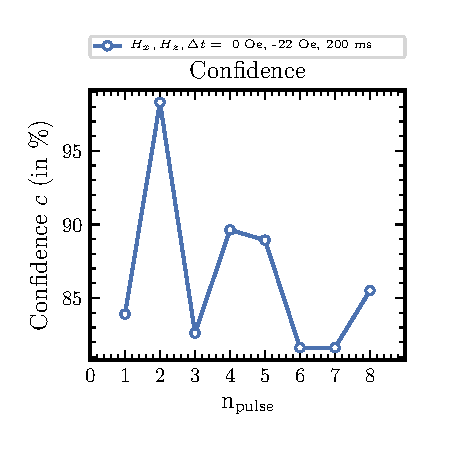
\includegraphics[scale=1.0]{figures/10_FitsSingleIteration/6__Confidence.pdf}\\
	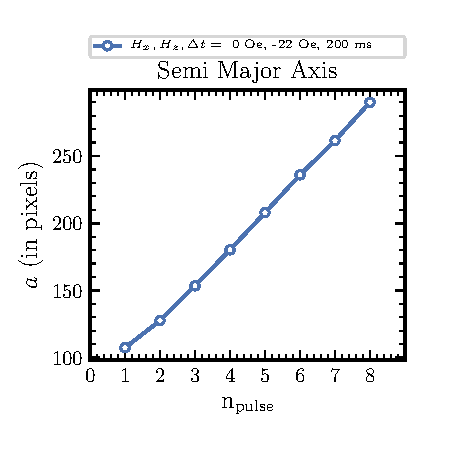
\includegraphics[scale=1.0]{figures/10_FitsSingleIteration/6__Semi-Major-Axis.pdf}
	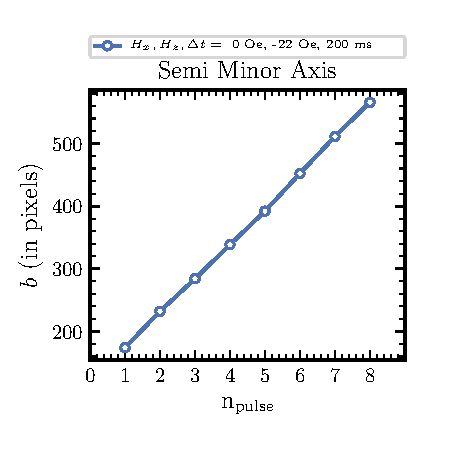
\includegraphics[scale=1.0]{figures/10_FitsSingleIteration/6__Semi-Minor-Axis.pdf}\\
	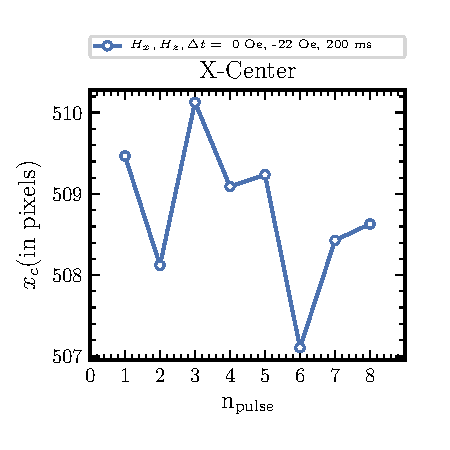
\includegraphics[scale=1.0]{figures/10_FitsSingleIteration/6__X-Center.pdf}
	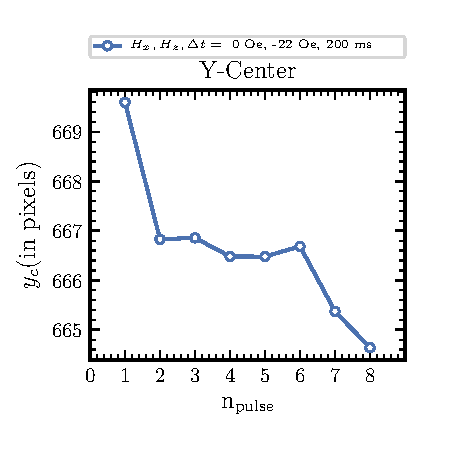
\includegraphics[scale=1.0]{figures/10_FitsSingleIteration/6__Y-Center.pdf}
	\caption{Parameters like confidence, center coordinates, semi major and minor axes and orientations for a sequence of pulses for a representative experiment sequence at $H_z = -22~\mathrm{Oe}, H_x = 0~\mathrm{Oe}$.
	}
	\label{openCV fits parameters single experiment}
\end{figure}
%

To cycle through all the experiments and plot the fits for each experiment run PlotExperimentIndices() in a loop for each experiment. The following code implements the iterations.
%
\begin{minted}[
frame=lines,
framesep=2mm,
baselinestretch=1.2,
bgcolor=lightgray,
fontsize=\footnotesize,
linenos
]{python}
if __name__ == '__main__':
filtered_experiments, controls_extracted, control_knobs = LoadFits()
n_exp = filtered_experiments.shape[1]
for i in np.arange(n_exp):
experiment_index = [i]
array_experiment_index = np.array(experiment_index)
PlotExperimentIndices(filtered_experiments, array_experiment_index, controls_extracted)
\end{minted}
%
\paragraph{Subspace of experiments}
Let us say we want to compare the information related to experiments $H_{z} = 10, 20, 30, 40~\mathrm{Oe}$, then we choose list of experiment indices $0, 5, 10, 15$ as shown below in code. Now to summarize the fit parameters for the experiments performed, let us draw surface plots for each of the parameters with x axis representing the pulse sequence and y-axis representing the experiment sequence. Also these subspace plots are saved at the top level of directory i.e. in the Fits subdirectory similar to where the total space of experiments is saved. In order to detect the files, the name of the file includes the indices included in the subspace. These subspace plots are shown in Figure.~\ref{openCV fit parameters some experiments}.
%
\begin{minted}[
frame=lines,
framesep=2mm,
baselinestretch=1.2,
bgcolor=lightgray,
fontsize=\footnotesize,
linenos
]{python}
if __name__ == '__main__':
filtered_experiments, controls_extracted, control_knobs = LoadFits()
list_experiment_index = [0, 5, 10, 15]
array_experiment_index = np.array(list_experiment_index)
PlotExperimentIndices(filtered_experiments, array_experiment_index, controls_extracted)
\end{minted}
%
%
\begin{figure}[!htbp]
	\centering
	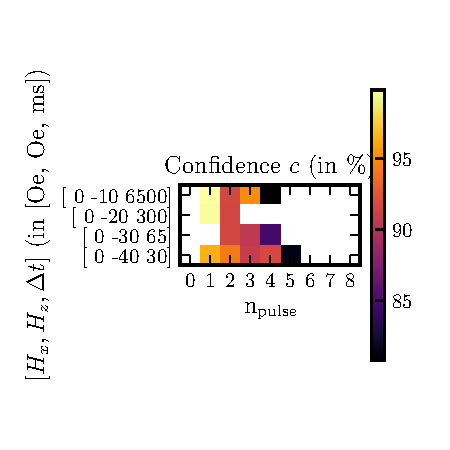
\includegraphics[scale=1.0]{figures/11_FitsSubSpace/0_5_10_15__Confidence.pdf}\\
	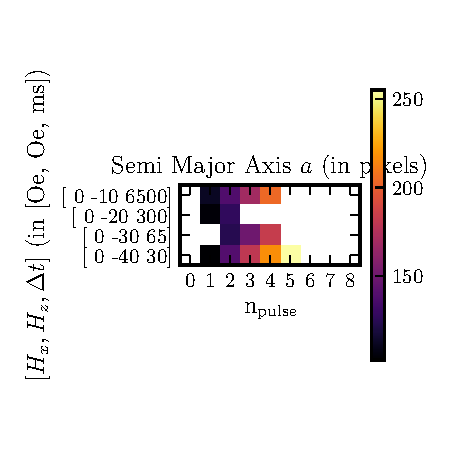
\includegraphics[scale=1.0]{figures/11_FitsSubSpace/0_5_10_15__Semi-Major-Axis.pdf}
	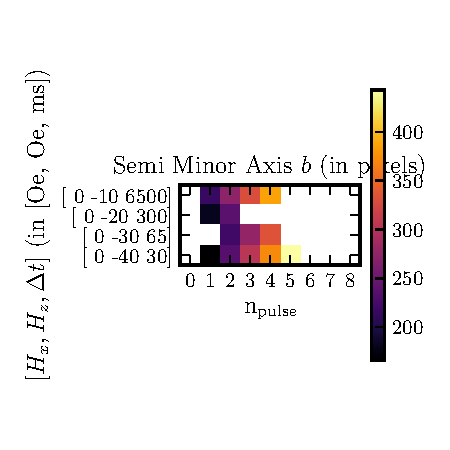
\includegraphics[scale=1.0]{figures/11_FitsSubSpace/0_5_10_15__Semi-Minor-Axis.pdf}
	\caption{Comparison of parameters for experiments corresponding to indices $0, 5, 10, 15$.
	}
	\label{openCV fit parameters some experiments}
\end{figure}
%

In similar way, to plot the whole experiment space, we can form the list of all the experiment indices and give as input to PlotExperimentIndices(). These are summarized in Figure.~\ref{openCV fit parameters all experiments}. To run these surface plots, we use the following code.
%
\begin{minted}[
frame=lines,
framesep=2mm,
baselinestretch=1.2,
bgcolor=lightgray,
fontsize=\footnotesize,
linenos
]{python}
if __name__ == '__main__':
filtered_experiments, controls_extracted, control_knobs = LoadFits()
# find the number of experiments
n_exp = filtered_experiments.shape[1]
array_experiment_index = np.arange(n_exp)
PlotExperimentIndices(filtered_experiments, array_experiment_index, controls_extracted)
\end{minted}
%
\begin{figure}[!htbp]
	\centering
	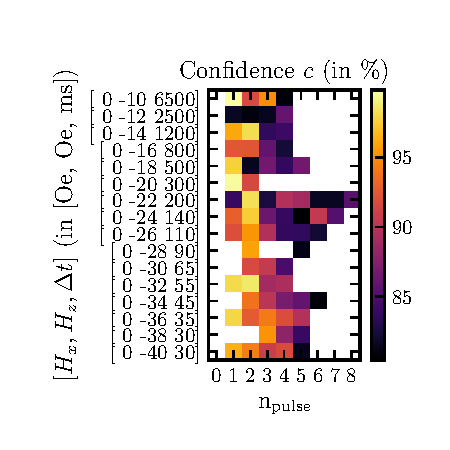
\includegraphics[scale=1.0]{figures/12_FitsFullSpace/0_1_2_3_4_5_6_7_8_9_10_11_12_13_14_15__Confidence.pdf}\\
	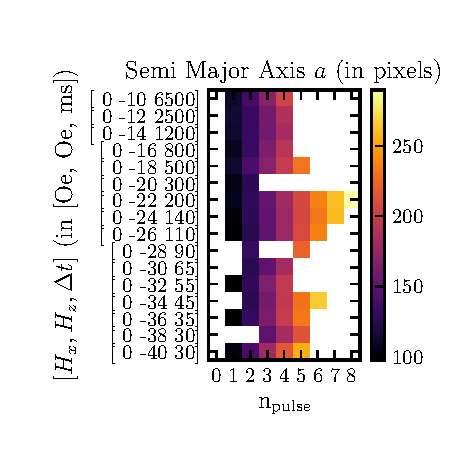
\includegraphics[scale=1.0]{figures/12_FitsFullSpace/0_1_2_3_4_5_6_7_8_9_10_11_12_13_14_15__Semi-Major-Axis.pdf}
	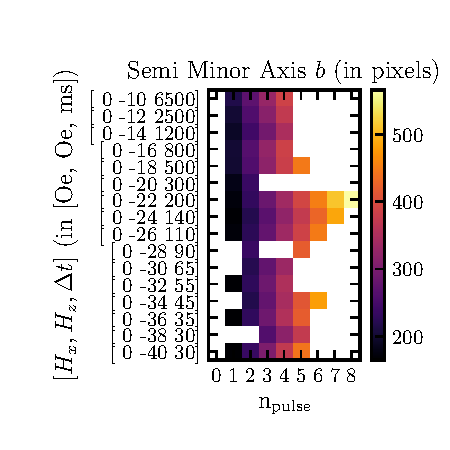
\includegraphics[scale=1.0]{figures/12_FitsFullSpace/0_1_2_3_4_5_6_7_8_9_10_11_12_13_14_15__Semi-Minor-Axis.pdf}\\
	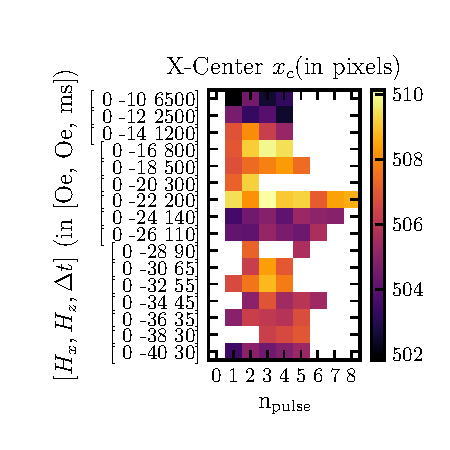
\includegraphics[scale=1.0]{figures/12_FitsFullSpace/0_1_2_3_4_5_6_7_8_9_10_11_12_13_14_15__X-Center.pdf}
	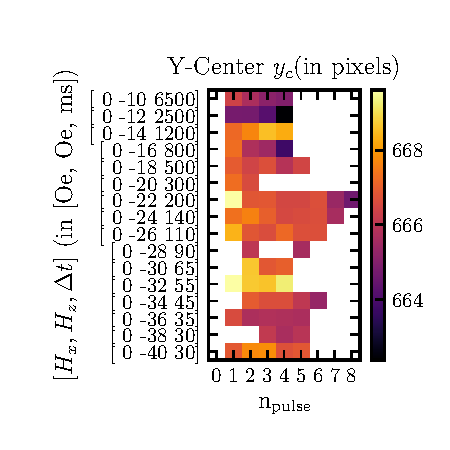
\includegraphics[scale=1.0]{figures/12_FitsFullSpace/0_1_2_3_4_5_6_7_8_9_10_11_12_13_14_15__Y-Center.pdf}
	\caption{Parameters like confidence, center coordinates, semi major and minor axes and orientations for a sequence of pulses for a representative experiment sequence at $H_z = -22~\mathrm{Oe}, H_x = 0~\mathrm{Oe}$.
	}
	\label{openCV fit parameters all experiments}
\end{figure}
%
\clearpage
\subsection{Velocity by experiment indices}
To estimated the velocity, we need to fit the shift of the center of bubble domain as well as the expansion of the major~(and minor) axes with pulse sequence to a linear fit. This is performed by \textbf{FindVelocityExperiment} routine
%
\begin{minted}[
frame=lines,
framesep=2mm,
baselinestretch=1.2,
bgcolor=lightgray,
fontsize=\footnotesize,
linenos
]{python}
def FindVelocityExperiment(experiment_index, experiments, goodfits, controls_extracted, DEBUG=True):
scale = 0.1/304 # in mm per pixel
factor = 1E6 # for velocity units in um/s
if DEBUG: print("Experiment is " + str(controls_extracted[experiment_index]))
velocity_center = np.zeros((1,2))
velocity_rel = np.zeros((1,2))
tp = controls_extracted[experiment_index][2]
if DEBUG: print("Experiment pulse width is " + str(tp))
goodfits_element = goodfits[experiment_index]
if DEBUG: print("goodfit element is " + str(goodfits_element))
goodfits_indices_element = np.nonzero(goodfits_element)
if DEBUG: print("good fit element index is " + str(goodfits_indices_element))
x = goodfits_indices_element[0]
cx = experiments[1][experiment_index][goodfits_indices_element[0]]
cy = experiments[2][experiment_index][goodfits_indices_element[0]]
a = experiments[3][experiment_index][goodfits_indices_element[0]]
b = experiments[4][experiment_index][goodfits_indices_element[0]]
if x.size < 2:  #then the the data is not sufficient to fit the line
if DEBUG: print("Data is not sufficient to extract the velocities!")
velocity_center[:] = np.nan
velocity_rel[:] = np.nan
else:
vc = np.transpose(np.asarray([cy,cx])) #swap the cx, cy to incorporate the difference in the coordinate system of image and the semi major and semi minor axis
ab = np.transpose(np.asarray([a, b]))
if DEBUG: print ("axes are :")
if DEBUG: print (x,ab)
if DEBUG: print ("centers are :")
if DEBUG: print (x,vc)
vel_center = np.polyfit(x,vc,1)
vel_rel = np.polyfit(x,ab,1)
velocity_center = vel_center[0]/tp*scale*factor
velocity_rel = vel_rel[0]/tp*scale*factor #slope of the polyfit (vel_rel[0]) is the displacement of the edge(in pixels) per pulse of field
if DEBUG: print ("Axes Velocity [[v_a v_b],...] in subspace of experiments is ")
if DEBUG: print (str(velocity_rel))
if DEBUG: print ("Center Velocity [[c_a c_b],...] in subspace of experiments is ")
if DEBUG: print (str(velocity_center))
return velocity_center, velocity_rel
\end{minted}
%
To run the velocity routine on all the experiments, we use \textbf{FindVelocityOnExperiments}
%
\begin{minted}[
frame=lines,
framesep=2mm,
baselinestretch=1.2,
bgcolor=lightgray,
fontsize=\footnotesize,
linenos
]{python}
def FindVelocityOnExperiments(experiments, goodfits, controls_extracted, debug=True):
"""Find the velocity on all the measurements which have good fits!!!"""
n_exp = controls_extracted.shape[0]
velocity_center =      np.zeros((n_exp,2)) # 2D array with columns corresponding to vx and vy of centers
velocity_rel    =      np.zeros((n_exp,2)) # 2D array with columns corresponding to vx and vy of axes
#iterate over each of the experiment and find the velocity
for i in np.arange(n_exp):
velocity_center[i],velocity_rel[i] = FindVelocityExperiment(i,experiments, goodfits, controls_extracted, debug)
return velocity_center, velocity_rel
\end{minted}
%
\clearpage



\subsection{DMI estimation}
To estimate Dzyaloshinksii Moriya interaction~(DMI), we need to find the velocity of the domain wall as a function of $H_z, H_x$.

%%%%%% bibliography
\addcontentsline{toc}{chapter}{Bibliography}

\bibliography{../../../myThesis/bibs/library}        %use a bibtex bibliography file refs.bib
\bibliographystyle{ieeetr}  %use the plain bibliography style
\end{document}